\documentclass[11pt,a4paper,oneside]{report}             % Single-side
%\documentclass[11pt,a4paper,twoside,openright]{report}  % Duplex

\PassOptionsToPackage{chapternumber=Huordinal}{magyar.ldf}
\usepackage{t1enc}
%\usepackage[latin2]{inputenc}
\usepackage[utf8]{inputenc}
\usepackage{amsmath}
\usepackage{amssymb}
\usepackage{enumerate}
\usepackage[thmmarks]{ntheorem}
\usepackage{graphics}
\usepackage{epsfig}
\usepackage{listings}
\usepackage{color}
%\usepackage{fancyhdr}
\usepackage{lastpage}
\usepackage{anysize}
\usepackage[magyar]{babel}
\usepackage{sectsty}
\usepackage{setspace}  % Ettol a tablazatok, abrak, labjegyzetek maradnak 1-es sorkozzel!
\usepackage[hang]{caption}
\usepackage{hyperref}
\usepackage{titlesec}
\usepackage{titletoc}

\usepackage{graphicx}
\usepackage{epstopdf}

\usepackage{amsmath,mathtools,calc}
%piramisrajzoláshoz
\usepackage{tikz}
\usetikzlibrary{intersections,decorations.pathreplacing,shapes.misc,calc,positioning}

%RUDI vektoros betűtípus
\usepackage{lmodern}
%\usepackage{newtxtext}
%--------------------------------------------------------------------------------------
% Main variables
%--------------------------------------------------------------------------------------
\newcommand{\vikszerzoI}{Ács Bence}
\newcommand{\vikszerzoII}{Jávorszky Zoltán}
\newcommand{\vikszerzoIII}{Medvedev Mihály}
\newcommand{\vikcim}{Stratégiai játék}
\newcommand{\viktanszek}{Beágyazott rendszerek szoftvertechnológiája}
\newcommand{\vikdoktipus}{Tervdokumentáció}
%\newcommand{\vikdepartmentr}{Bódis-Szomorú András}

%--------------------------------------------------------------------------------------
% Page layout setup
%--------------------------------------------------------------------------------------
% we need to redefine the pagestyle plain
% another possibility is to use the body of this command without \fancypagestyle
% and use \pagestyle{fancy} but in that case the special pages
% (like the ToC, the References, and the Chapter pages)remain in plane style

\pagestyle{plain}
%\setlength{\parindent}{0pt} % áttekinthetõbb, angol nyelvû dokumentumokban jellemzõ
%\setlength{\parskip}{8pt plus 3pt minus 3pt} % áttekinthetõbb, angol nyelvû dokumentumokban jellemzõ
\setlength{\parindent}{12pt} % magyar nyelvû dokumentumokban jellemzõ
\setlength{\parskip}{0pt}    % magyar nyelvû dokumentumokban jellemzõ

\marginsize{35mm}{25mm}{15mm}{15mm} % anysize package
\setcounter{secnumdepth}{1}
\sectionfont{\large\upshape\bfseries}
\setcounter{secnumdepth}{1}
\singlespacing
\frenchspacing

\titleformat{\chapter}[display]
{\normalfont\huge\bfseries}{}{0pt}{\Huge}
\renewcommand\thesection{\arabic{section}}

\titlecontents{chapter}
[0em]{\addvspace{10pt}\bfseries}
{}{}{\titlerule*[1000pc]{.}\contentspage}

\usepackage{tabularx}
\usepackage{longtable}
\usepackage{tabu}

%--------------------------------------------------------------------------------------
%	Setup hyperref package
%--------------------------------------------------------------------------------------
\hypersetup{
    bookmarks=true,            % show bookmarks bar?
    unicode=false,             % non-Latin characters in Acrobat’s bookmarks
    pdftitle={\vikcim},        % title
    pdfauthor={\vikszerzoI,\vikszerzoII,\vikszerzoIII},    % author
    pdfsubject={\vikdoktipus}, % subject of the document
    pdfcreator={\vikszerzoI},   % creator of the document
    pdfproducer={Producer},    % producer of the document
    pdfkeywords={keywords},    % list of keywords
    pdfnewwindow=true,         % links in new window
    colorlinks=true,           % false: boxed links; true: colored links
    linkcolor=black,           % color of internal links
    citecolor=black,           % color of links to bibliography
    filecolor=black,           % color of file links
    urlcolor=black             % color of external links
}

%--------------------------------------------------------------------------------------
% Set up listings
%--------------------------------------------------------------------------------------
%\lstset{language=C}
\lstset{
	basicstyle=\scriptsize\ttfamily, % print whole listing small
	keywordstyle=\color{black}\bfseries\underbar, % underlined bold black keywords
	identifierstyle=, 					% nothing happens
	commentstyle=\color{white}, % white comments
	stringstyle=\scriptsize\sffamily, 			% typewriter type for strings
	showstringspaces=false,     % no special string spaces
	aboveskip=3pt,
	belowskip=3pt,
	columns=fixed,
	backgroundcolor=\color{lightgray},
	inputencoding=utf8,
	extendedchars=true,
	literate={á}{{\'a}}1 {ã}{{\~a}}1 {é}{{\'e}}1,
} 		
\def\lstlistingname{lista}	

%--------------------------------------------------------------------------------------
%	Some new commands and declarations
%--------------------------------------------------------------------------------------
\newcommand{\code}[1]{{\upshape\ttfamily\scriptsize\indent #1}}

% define references
\newcommand{\figref}[1]{\ref{fig:#1}.}
\renewcommand{\eqref}[1]{(\ref{eq:#1})}
\newcommand{\listref}[1]{\ref{listing:#1}.}
\newcommand{\sectref}[1]{\ref{sect:#1}}
\newcommand{\tabref}[1]{\ref{tab:#1}.}

\DeclareMathOperator*{\argmax}{arg\,max}
%\DeclareMathOperator*[1]{\floor}{arg\,max}
\DeclareMathOperator{\sign}{sgn}
\DeclareMathOperator{\rot}{rot}
\definecolor{lightgray}{rgb}{0.95,0.95,0.95}

\author{\vikszerzo}
\title{\viktitle}
\includeonly{
	%guideline,%
	%project,%
	titlepage,%
%	declaration,%
%	abstract,%
%	introduction,%
	chapter1,%
	chapter2,%
	chapter3,%
%	acknowledgement,%
%	appendices,%
}
%--------------------------------------------------------------------------------------
%	Setup captions
%--------------------------------------------------------------------------------------
\captionsetup[figure]{
%labelsep=none,
%font={footnotesize,it},
%justification=justified,
width=.75\textwidth,
aboveskip=10pt}

\renewcommand{\captionlabelfont}{\small\bf}
\renewcommand{\captionfont}{\footnotesize\it}

%
\newcommand{\fname}[1]{\mbox{\texttt{#1}}}

%--------------------------------------------------------------------------------------
% Table of contents and the main text
%--------------------------------------------------------------------------------------
\begin{document}
\singlespacing
%\include{guideline}
%\include{project}

\pagenumbering{arabic}
\onehalfspacing
%--------------------------------------------------------------------------------------
%	The title page
%--------------------------------------------------------------------------------------
\begin{titlepage}
\begin{center}

\includegraphics[width=60mm,keepaspectratio]{figures/BMElogo.png}\\
\vspace{0.3cm}
\textbf{Budapesti Mûszaki és Gazdaságtudományi Egyetem}\\
\textmd{Villamosmérnöki és Informatikai Kar}\\
\textmd{\viktanszek}\\[5cm]

\vspace{0.4cm}
{\huge \bfseries \vikcim}\\[0.8cm]
\vspace{0.5cm}
\textsc{\Large \vikdoktipus}\\[4cm]

\begin{tabular}{cc}
 \makebox[14cm]{\emph{Készítette}}\\
 \makebox[7cm]{\vikszerzoI}\\
 \makebox[7cm]{\vikszerzoII}\\
 \makebox[7cm]{\vikszerzoIII}
\end{tabular}

\vfill
{\large \today}
\end{center}
\end{titlepage}



\tableofcontents\vfill
%----------------------------------------------------------------------------
%\chapter{\LaTeX-eszközök}\label{sect:LatexTools}
%----------------------------------------------------------------------------
\section{Általános leírás}
%----------------------------------------------------------------------------
A megvalósítani kívánt játék egy körökre osztott stratégiai játék, mely során egy harctéren különböző fajú karakterekkel harcolnak a játékosok.
A karakterek a játék előtt meghatározott felszerelést visznek magukkal, melyeket felhasználhatják a harc során. Körönként egy karakter egyet lép, majd egy kisorsolt felszerelést felhasznál. A játék addig tart, amíg már csak egy játékos karaktere(i) marad(nak) életben.


%----------------------------------------------------------------------------
\section{A játék menete}
%----------------------------------------------------------------------------
\begin{enumerate}
	\item Egyik játékos elindítja a Servert, a másik (többi) kliensként csatlakozik.
	\item Server játékos beállítja a játék paramétereit.
	\begin{itemize}\label{StartParams}
		\item Maximális játékos szám, maximális karakter száma játékosonként.
		\item Maximális pályaméret(szélesség és magasság).
		\item Használható karakter fajok
		\begin{itemize}
			\item Azok számai fajonként
			\item Azok szintjei
		\end{itemize}
	\end{itemize}
	\item Játékosok kiválasztják a használandó karaktereket, majd beállítják azok felszereléseit, jelzik, ha készen vannak.
	\item Ha mindenki készen áll, akkor a szerver legenerálja a pályát. A generált pályára a játékosok elhelyezik a karaktereket. Ha ez megtörténik indul a harc.
\end{enumerate}


%----------------------------------------------------------------------------
\section{A harc menete}
%----------------------------------------------------------------------------
\begin{enumerate}
\item A szerver felállít egy sorrendet a játékosok között. A karakter fajokon végighaladva következnek a játékosok

\newcommand{\owntabnr}{4cm}
\newcommand{\colwid}{\textwidth-\owntabnr)/6}
\begin{tabular}{ |p{(\colwid}|p{(\colwid}|p{(\colwid}|p{(\colwid}|p{(\colwid}|p{(\colwid}|  }
	\hline
	\multicolumn{6}{|c|}{Példa} \\
	\hline
	\multicolumn{2}{|c|}{Lovag}& \multicolumn{2}{|c|}{Íjász} & \multicolumn{2}{|c|}{Mágus} \\
	\hline
	1. játékos lovagjai & 2. játékos lovagjai & 1. játékos lovagjai & 2. játékos lovagjai  & 1. játékos mágusa & 2. játékos mágusa \\
	\hline
\end{tabular}
\item A sorra kerülő karakter a 8 szomszédos mező egyikére lép, majd a rendszer a beállított felszerelések közül kisorsol egyet, melyet a játék felhasznál. (támadásnál a támadott ellenfelet is ki kell választani)
\item A játék addig tart, amíg már csak egy játékos karaktere(i) marad(nak) életben.
\end{enumerate}


%----------------------------------------------------------------------------
\section{A menürendszer}
%----------------------------------------------------------------------------


%----------------------------------------------------------------------------
\section{A játéktér}
%----------------------------------------------------------------------------
\begin{itemize}
	\item A harctér egy Descartes-féle derékszögű koordináta rendszer, melyben az elemek pozíciója csak egész szám lehet. ($x,y \epsilon Z  $)
	\item A harcteret a servert futtató játékos szoftvere generálja, az általa beállított \hyperref[StartParams]{\textit{paramétereknek}} megfelelően.
	\begin{itemize}
		\item Egy játékmező lehet érinthető/nem érinthető.
		\item Egy összefüggő területre (maximális N mezőre) egy dedikált játékos maximum k karaktert rakhat.
	\end{itemize}
	\item A harctéren egy mezőn, egyszerre csak egy karakter állhat.
\end{itemize}


%----------------------------------------------------------------------------
\section{Karakter}
%----------------------------------------------------------------------------
\begin{itemize}
	\item Egy karakter egy harc alatt maximum 6 felszerelést (egy fajtából akár többet is) választhat magának.
	\item A játék elején megadott karakter szint meghatározza a választható felszereléseket.
	\item A felszerelések értékei változóak, a karakterekhez tartozó összértékek a játék elején megadott paraméterekkel korlátozhatóak.
	\item A karaktereknek fajai vannak, melyek a következőek:	
	\begin{itemize}
		\item Lovag
		\item Íjász
		\item Mágus
	\end{itemize} 
\end{itemize}



%----------------------------------------------------------------------------
\section{Felszerelés}
%----------------------------------------------------------------------------

\begin{longtabu} to \textwidth {X[2l]|X[1.5l]|X[1.2c]|X[1.3c]|X[5l]}
	\rowfont[c]{\small}Név           & Faj     & Minimum Szint & Felhasznált érték & Leírás                                                                 \\ \hline \endhead
	Fa kard       & Bármelyik & 1             & 1                 & Egy szomszédos ellenfelet támad 1 erősséggel.                          \\
	Fa pajzs      & Bármelyik & 1             & 1                 & Megvéd az 1 erősségű támadások ellen.                                  \\
	Vas kard      & Lovag     &               & 2                 & Egy szomszédos ellenfelet támad 2 erősséggel.                          \\
	Pörgő fa kard & Lovag     &               & 2                 & Az összes szomszédos ellenfelet támadja 1 erősséggel.                  \\
	Tőr           & Lovag     &               & 2                 & Ismét léphet egyet, majd egy szomszédos ellenfelet támad 1 erősséggel. \\
	Vas pajzs& Lovag          &               & 2                  &  Megvéd a 2 erősségű támadások ellen.                                                                  \\
	Helytállás pengéje& Lovag          &               &  2                 & Egy szomszédos ellenfelet támad 1 erősséggel és megvéd az 1 erősségű támadások ellen.                                                                        \\
	&           &               &                   &                                                                        \\
	&           &               &                   &                                                                        \\
	&           &               &                   &   
\end{longtabu}
%%----------------------------------------------------------------------------
\chapter{A dolgozat formai kivitele}
%----------------------------------------------------------------------------
Az itt található információk egy része a BME VIK Hallgatói Képviselet által készített ,,Utolsó félév a villanykaron'' c. munkából lett kis változtatásokkal átemelve. Az eredeti dokumentum az alábbi linken érhetõ el: \url{http://vik-hk.bme.hu/diplomafelev-howto-2009}.

%----------------------------------------------------------------------------
\section{A dolgozat kimérete}
%----------------------------------------------------------------------------
A minimális 50, az optimális kiméret 60-70 oldal (függelékkel együtt). A bírálók és a záróvizsga bizottság sem szereti kifejezetten a túl hosszú dolgozatokat, így a bruttó 90 oldalt már nem érdemes túlszárnyalni. Egyébként függetlenül a dolgozat kiméretétõl, ha a dolgozat nem érdekfeszítõ, akkor az olvasó már az elején a végét fogja várni. Érdemes zárt, önmagában is érthetõ mûvet alkotni.

%----------------------------------------------------------------------------
\section{A dolgozat nyelve}
%----------------------------------------------------------------------------
Mivel Magyarországon a hivatalos nyelv a magyar, ezért alapértelmezésben magyarul kell megírni a dolgozatot. Aki külföldi posztgraduális képzésben akar részt venni, nemzetközi szintû tudományos kutatást szeretne végezni, vagy multinacionális cégnél akar elhelyezkedni, annak célszerû angolul megírnia diplomadolgozatát. Mielõtt a hallgató az angol nyelvû verzió mellett dönt, erõsen ajánlott mérlegelni, hogy ez mennyi többletmunkát fog a hallgatónak jelenteni fogalmazás és nyelvhelyesség terén, valamint - nem utolsó sorban - hogy ez mennyi többletmunkát fog jelenteni a konzulens illetve bíráló számára. Egy nehezen olvasható, netalán érthetetlen szöveg teher minden játékos számára.

%----------------------------------------------------------------------------
\section{A dokumentum nyomdatechnikai kivitele}
%----------------------------------------------------------------------------
A dolgozatot A4-es fehér lapra nyomtatva, 2,5 centiméteres margóval (+1~cm kötésbeni), 11-12 pontos betûmérettel, talpas betûtípussal és másfeles sorközzel célszerû elkészíteni.



%%----------------------------------------------------------------------------
%\chapter{A \LaTeX-sablon használata}
%----------------------------------------------------------------------------
Ebben a fejezetben röviden, implicit módon bemutatjuk a sablon használatának módját, ami azt jelenti, hogy sablon használata ennek a dokumentumnak a forráskódját tanulmányozva válik teljesen világossá. Amennyiben a szoftver-keretrendszer telepítve van, a sablon alkalmazása és a dolgozat szerkesztése \LaTeX-ben a sablon segítségével tapasztalataink szerint jóval hatékonyabb, mint egy WYSWYG (\emph{What You See is What You Get}) típusú szövegszerkesztõ esetén (pl. Microsoft Word, OpenOffice).

%----------------------------------------------------------------------------
\section{Címkék és hivatkozások}
%----------------------------------------------------------------------------
A \LaTeX~dokumentumban címkéket (\verb+\label+) rendelhetünk ábrákhoz, táblázatokhoz, fejezetekhez, listákhoz, képletekhez stb. Ezekre a dokumentum bármely részében hivatkozhatunk, a hivatkozások automatikusan feloldásra kerülnek.

A sablonban makrókat definiáltunk a hivatkozások megkönnyítéséhez. Ennek megfelelõen minden ábra (\emph{figure}) címkéje \verb+fig:+ kulcsszóval kezdõdik, míg minden táblázat (\emph{table}), képlet (\emph{equation}), fejezet (\emph{section}) és lista (\emph{listing}) rendre a \verb+tab:+, \verb+eq:+, \verb+sect:+ és \verb+listing:+ kulcsszóval kezdõdik, és a kulcsszavak után tetszõlegesen választott címke használható. Ha ezt a konvenciót betartjuk, akkor az elõbbi objektumok számára rendre a \verb+\figref+, \verb+\tabref+, \verb+\eqref+, \verb+\sectref+ és \verb+\listref+ makrókkal hivatkozhatunk. A makrók paramétere a címke, amelyre hivatkozunk (a kulcsszó nélkül). Az összes említett hivatkozástípus, beleértve az \verb+\url+ kulcsszóval bevezetett web-hivatkozásokat is a  \verb+hyperref+\footnote{Segítségével a dokumentumban megjelenõ hivatkozások nem csak dinamikussá válnak, de színezhetõk is, bõvebbet errõl a csomag dokumentációjában találunk. Ez egyúttal egy példa lábjegyzet írására.} csomagnak köszönhetõen aktívak a legtöbb PDF-nézegetõben, rájuk kattintva a dokumentum megfelelõ oldalára ugrik a PDF-nézõ vagy a megfelelõ linket megnyitja az alapértelmezett böngészõvel. A \verb+hyperref+ csomag a kimeneti PDF-dokumentumba könyvjelzõket is készít a tartalomjegyzékbõl. Ez egy szintén aktív tartalomjegyzék, amelynek elemeire kattintva a nézegetõ behozza a kiválasztott fejezetet.

%----------------------------------------------------------------------------
\section{Ábrák és táblázatok}
%----------------------------------------------------------------------------
A képeket PDFLaTeX esetén a veszteségmentes PNG, valamint a veszteséges JPEG formátumban érdemes elmenteni. Az EPS (PostScript) vektorgrafikus képformátum beillesztését a PDFLatex közvetlenül nem támogatja. Ehelyett egy lehetõség 200 dpi, vagy annál nagyobb felbontásban raszterizálni a képet, és PNG formátumban elmenteni. Az egyes képek mérete általában nem, de sok kép esetén a dokumentum összmérete így már szignifikáns is lehet. A dokumentumban felhasznált képfájlokat a dokumentum forrása mellett érdemes tartani, archiválni, mivel ezek hiányában a dokumentum nem fordul újra. Ha lehet, a vektorgrafikus képeket vektorgrafikus formátumban is érdemes elmenteni az újrafelhasználhatóság (az átszerkeszthetõség) érdekében.

Kapcsolási rajzok legtöbbször kimásolhatók egy vektorgrafikus programba (pl. CorelDraw) és onnan nagyobb felbontással raszterizálva kimenthatõk PNG formátumban. Ugyanakkor kiváló ábrák készíthetõk Microsoft Visio vagy hasonló program használatával is: Visio-ból az ábrák közvetlenül PNG-be is menthetõk.

Lehetõségeink Matlab ábrák esetén:
\begin{itemize}
	\item Képernyõlopás (\emph{screenshot}) is elfogadható minõségû lehet a dokumentumban, de általában jobb felbontást is el lehet érni más módszerrel.
	\item A Matlab ábrát a \verb+File/Save As+ opcióval lementhetjük PNG formátumban (ugyanaz itt is érvényes, mint korábban, ezért nem javasoljuk).
	\item A Matlab ábrát az \verb+Edit/Copy figure+ opcióval kimásolhatjuk egy vektorgrafikus programba is és onnan nagyobb felbontással raszterizálva kimenthatjük PNG formátumban (nem javasolt).
	\item Javasolt megoldás: az ábrát a \verb+File/Save As+ opcióval EPS \emph{vektorgrafikus} formátumban elmentjük, PDF-be konvertálva beillesztjük a dolgozatba.
\end{itemize}
Az EPS kép az \verb+epstopdf+ programmal\footnote{a korábban említett \LaTeX-disztribúciókban megtalálható} konvertálható PDF formátumba. Célszerû egy batch-fájlt készíteni az összes EPS ábra lefordítására az alábbi módon (ez Windows alatt mûködik).
\begin{lstlisting}[frame=single,float=!ht]
@echo off
for %%j in (*.eps) do (
echo converting file "%%j"
epstopdf "%%j"
)
echo done .
\end{lstlisting}

Egy ilyen parancsfájlt (\verb+convert.cmd+) elhelyeztük a sablon \verb+figures\eps+ könyvtárába, így a felhasználónak csak annyi a dolga, hogy a \verb+figures\eps+ könyvtárba kimenti az EPS formátumú vektorgrafikus képet, majd lefuttatja a \verb+convert.cmd+ parancsfájlt, ami PDF-be konvertálja az EPS fájlt.

Ezek után a PDF-ábrát ugyanúgy lehet a dokumentumba beilleszteni, mint a PNG-t vagy a JPEG-et. A megoldás elõnye, hogy a lefordított dokumentumban is vektorgrafikusan tárolódik az ábra, így a mérete jóval kisebb, mintha raszterizáltuk volna beillesztés elõtt. Ez a módszer minden -- az EPS formátumot ismerõ -- vektorgrafikus program (pl. CorelDraw) esetén is használható.

A képek beillesztésére az \sectref{LatexTools}. fejezetben mutattunk be példát (\figref{TexnicCenter}~ábra). Az elõzõ mondatban egyúttal az automatikusan feloldódó ábrahivatkozásra is láthatunk példát. Több képfájlt is beilleszthetünk egyetlen ábrába. Az egyes képek közötti horizontális és vertikális margót metrikusan szabályozhatjuk (\figref{HVSpaces}~ábra). Az ábrák elhelyezését számtalan tipográfiai szabály egyidejû teljesítésével a fordító maga végzi, a dokumentum írója csak preferenciáit jelezheti a fordító felé (olykor ez bosszúságot is okozhat, ilyenkor pl. a kép méretével lehet játszani).

\begin{figure}[!ht]
\centering
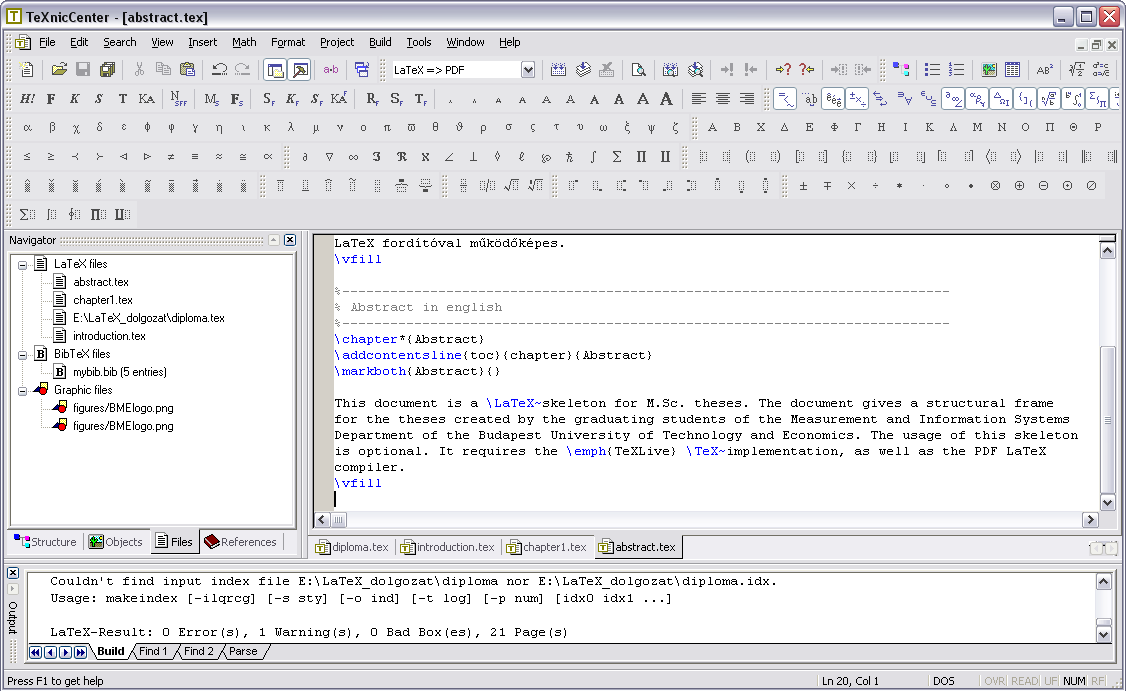
\includegraphics[width=67mm, keepaspectratio]{figures/TeXnicCenter.png}\hspace{1cm}
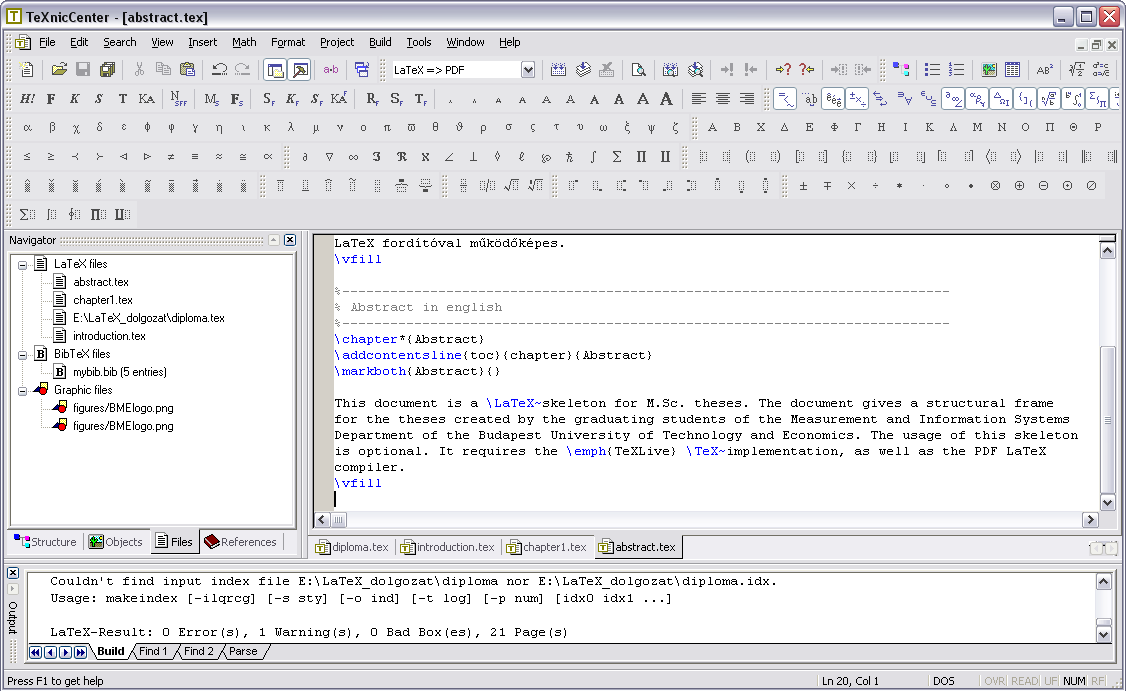
\includegraphics[width=67mm, keepaspectratio]{figures/TeXnicCenter.png}\\\vspace{5mm}
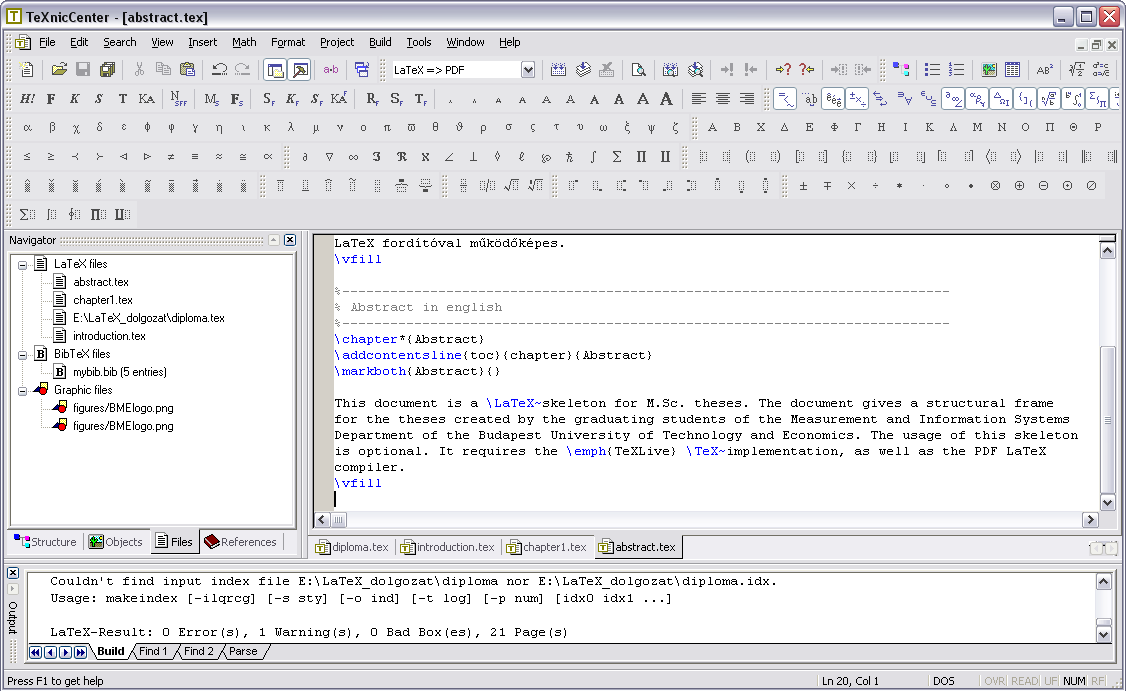
\includegraphics[width=67mm, keepaspectratio]{figures/TeXnicCenter.png}\hspace{1cm}
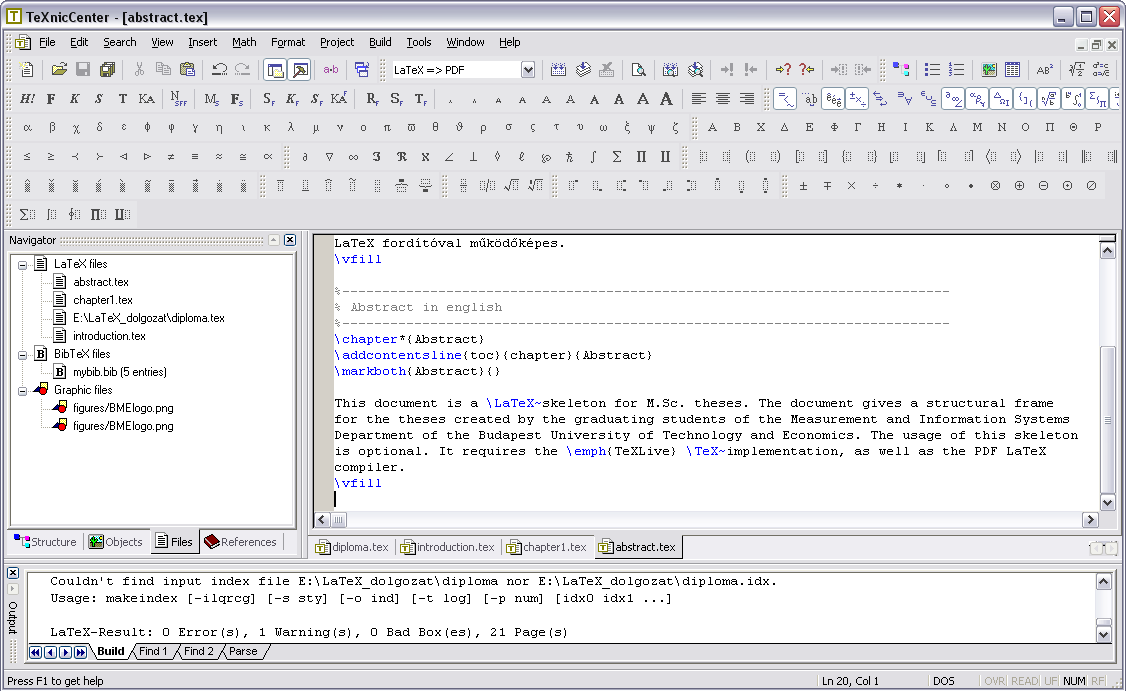
\includegraphics[width=67mm, keepaspectratio]{figures/TeXnicCenter.png}
\caption{Több képfájl beillesztése esetén térközöket is érdemes használni.} 
\label{fig:HVSpaces}
\end{figure}

A táblázatok használatára a \tabref{TabularExample}~táblázat mutat példát.
A táblázat címkéje nem véletlenül került a táblázat fölé, ez a szokványos.
\begin{table}[ht]
	\footnotesize
	\centering
	\caption{Az órajel-generátor chip órajel-kimenetei.} \label{tab:SysClocks}
	\begin{tabular}{ | l | c | c |}
	\hline
	Órajel & Frekvencia & Cél pin \\ \hline
	CLKA & 100 MHz & FPGA CLK0\\
	CLKB & 48 MHz  & FPGA CLK1\\
	CLKC & 20 MHz  & Processzor\\
	CLKD & 25 MHz  & Ethernet chip \\
	CLKE & 72 MHz  & FPGA CLK2\\
	XBUF & 20 MHz  & FPGA CLK3\\
	\hline
	\end{tabular}
	\label{tab:TabularExample}
\end{table}


%----------------------------------------------------------------------------
\section{Felsorolások és listák}
%----------------------------------------------------------------------------
Számozatlan felsorolásra mutat példát a jelenlegi bekezdés:
\begin{itemize}
	\item \emph{elsõ bajusz:} ide lehetne írni az elsõ elem kifejését,
	\item \emph{második bajusz:} ide lehetne írni a második elem kifejését,
	\item \emph{ez meg egy szakáll:} ide lehetne írni a harmadik elem kifejését.
\end{itemize}

Számozott felsorolást is készíthetünk az alábbi módon:
\begin{enumerate}
	\item \emph{elsõ bajusz:} ide lehetne írni az elsõ elem kifejését, és ez a kifejtés így néz ki, ha több sorosra sikeredik,
	\item \emph{második bajusz:} ide lehetne írni a második elem kifejését,
	\item \emph{ez meg egy szakáll:} ide lehetne írni a harmadik elem kifejését.
\end{enumerate}
A felsorolásokban sorok végén vesszõ, az utolsó sor végén pedig pont a szokásos írásjel. Ez alól kivételt képezhet, ha az egyes elemek több teljes mondatot tartalmaznak.

Listákban a dolgozat szövegétõl elkülönítendõ kódrészleteket, programsorokat, pszeudo-kódokat jeleníthetünk meg (\listref{Example}~lista). 
\begin{lstlisting}[frame=single,float=!ht,caption=A fenti számozott felsorolás \LaTeX- forráskódja, label=listing:Example]

\end{lstlisting}
A lista keretét, háttérszínét, egész stílusát megválaszthatjuk. Ráadásul különféle programnyelveket és a nyelveken belül kulcsszavakat is definiálhatunk, ha szükséges. Errõl bõvebbet a \verb+listings+ csomag hivatalos leírásában találhatunk.

%----------------------------------------------------------------------------
\section{Képletek}
%----------------------------------------------------------------------------
Ha egy formula nem túlságosan hosszú, és nem akarjuk hivatkozni a szövegbõl, mint például a $e^{i\pi}+1=0$ képlet, \emph{szövegközi képletként} szokás leírni. Csak, hogy másik példát is lássunk, az $U_i=-d\Phi/dt$ Faraday-törvény a $\rot E=-\frac{dB}{dt}$ differenciális alakban adott Maxwell-egyenlet felületre vett integráljából vezethetõ le. Látható, hogy a \LaTeX-fordító a sorközöket betartja, így a szöveg szedése esztétikus marad szövegközi képletek használata esetén is.

Képletek esetén az általános konvenció, hogy a kisbetûk skalárt, a kis félkövér betûk ($\mathbf{v}$) oszlopvektort -- és ennek megfelelõen $\mathbf{v}^T$ sorvektort -- a kapitális félkövér betûk ($\mathbf{V}$) mátrixot jelölnek. Ha ettõl el szeretnénk térni, akkor az alkalmazni kívánt jelölésmódot célszerû külön alfejezetben definiálni. Ennek megfelelõen, amennyiben $\mathbf{y}$ jelöli a mérések vektorát, $\mathbf{\vartheta}$ a paraméterek vektorát és $\hat{\mathbf{y}}=\mathbf{X}\vartheta$ a paraméterekben lineáris modellt, akkor a \emph{Least-Squares} értelemben optimális paraméterbecslõ $\hat{\mathbf{\vartheta}}_{LS}=(\mathbf{X}^T\mathbf{X})^{-1}\mathbf{X}^T\mathbf{y}$ lesz.

Emellett kiemelt, sorszámozott képleteket is megadhatunk, ennél az \verb+equation+ és a \verb+eqnarray+ környezetek helyett a korszerûbb \verb+align+ környezet alkalmazását javasoljuk (több okból, különféle problémák elkerülése végett, amelyekre most nem térünk ki). Tehát
\begin{align}
\dot{\mathbf{x}}&=\mathbf{A}\mathbf{x}+\mathbf{B}\mathbf{u},\\
\mathbf{y}&=\mathbf{C}\mathbf{x},
\end{align}
ahol $\mathbf{x}$ az állapotvektor, $\mathbf{y}$ a mérések vektora és $\mathbf{A}$, $\mathbf{B}$ és $\mathbf{C}$ a rendszert leíró paramétermátrixok. Figyeljük meg, hogy a két egyenletben az egyenlõségjelek egymáshoz igazítva jelennek meg, mivel a mindkettõt az \& karakter elõzi meg a kódban. Lehetõség van számozatlan kiemelt képlet használatára is, például
\begin{align}
\dot{\mathbf{x}}&=\mathbf{A}\mathbf{x}+\mathbf{B}\mathbf{u},\nonumber\\
\mathbf{y}&=\mathbf{C}\mathbf{x}\nonumber.
\end{align}
Mátrixok felírására az $\mathbf{A}\mathbf{x}=\mathbf{b}$ inhomogén lineáris egyenlet részletes kifejtésével mutatunk példát:
\begin{align}
\begin{bmatrix}
a_{11} & a_{12} & \dots & a_{1n}\\
a_{21} & a_{22} & \dots & a_{2n}\\
\vdots & \vdots & \ddots & \vdots\\
a_{m1} & a_{m2} & \dots & a_{mn}
\end{bmatrix}
\begin{pmatrix}x_1\\x_2\\\vdots\\x_n\end{pmatrix}=
\begin{pmatrix}b_1\\b_2\\\vdots\\b_m\end{pmatrix}.
\end{align}
A \verb+\frac+ utasítás hatékonyságát egy általános másodfokú tag átviteli függvényén keresztül mutatjuk be, azaz
\begin{align}
W(s)=\frac{A}{1+2T\xi s+s^2T^2}.
\end{align}
A matematikai mód minden szimbólumának és képességének a bemutatására természetesen itt nincs lehetõség, de gyors referenciaként hatékonyan használhatók a következõ linkek:\\
\indent\url{http://www.artofproblemsolving.com/LaTeX/AoPS_L_GuideSym.php},\\
\indent\url{http://www.ctan.org/tex-archive/info/symbols/comprehensive/symbols-a4.pdf},\\
\indent\url{ftp://ftp.ams.org/pub/tex/doc/amsmath/short-math-guide.pdf}.\\
Ez pedig itt egy magyarázat, hogy miért érdemes \verb+align+ környezetet használni:\\
\indent\url{http://texblog.net/latex-archive/maths/eqnarray-align-environment/}.

%----------------------------------------------------------------------------
\section{Irodalmi hivatkozások}\label{sect:HowtoReference}
%----------------------------------------------------------------------------
Egy \LaTeX dokumentumban az irodalmi hivatkozások definíciójának két módja van. Az egyik a \verb+\thebibliograhy+ környezet használata a dokumentum végén, az \verb+\end{document}+ lezárás elõtt.
\begin{lstlisting}[frame=single,float=!ht]
\begin{thebibliography}{9}

\bibitem{Lamport94} Leslie Lamport, \emph{\LaTeX: A Document Preparation System}. 
Addison Wesley, Massachusetts, 2nd Edition, 1994.

\end{thebibliography}
\end{lstlisting}

Ezek után a dokumentumban a \verb+\cite{Lamport94}+ utasítással hivatkozhatunk a forrásra. A fenti megadás viszonylag kötetlen, a szerzõ maga formázza az irodalomjegyzéket. 

Egy sokkal professzionálisabb módszer a BiB\TeX~használata, ezért ez a sablon is ezt támogatja. Ebben az esetben egy külön szöveges adatbázisban definiáljuk a forrásmunkákat, és egy külön stílusfájl határozza meg az irodalomjegyzék kinézetét. Ez, összhangban azzal, hogy külön formátumkonvenció határozza meg a folyóirat-, a könyv-, a konferenciacikk- stb. hivatkozások kinézetét az irodalomjegyzékben (a sablon használata esetén ezzel nem is kell foglalkoznia a hallgatónak, de az eredményt célszerû ellenõrizni). A felhasznált hivatkozások adatbázisa egy \verb+.bib+ kiterjesztésû szöveges fájl, amelynek szerkezetét a \listref{Bibtex} kódrészlet demonstrálja. A forrásmunkák bevitelekor a sor végi vesszõk külön figyelmet igényelnek, mert hiányuk a BiB\TeX-fordító hibaüzenetét eredményezi. A forrásmunkákat típus szerinti kulcsszó vezeti be (\verb+@book+ könyv, \verb+@inproceedings+ konferenciakiadványban megjelent cikk, \verb+@article+ folyóiratban megjelent cikk, \verb+@techreport+ valamelyik egyetem gondozásában megjelent mûszaki tanulmány, \verb+@manual+ mûszaki dokumentáció esetén stb.). Nemcsak a megjelenés stílusa, de a kötelezõen megadandó mezõk is típusról-típusra változnak. Egy jól használható referencia a \url{http://en.wikipedia.org/wiki/BibTeX} oldalon található.
\begin{lstlisting}[frame=single,float=!ht,caption=Példa szöveges irodalomjegyzék-adatbázisra BiBTeX használata esetén., label=listing:Bibtex]

\end{lstlisting}

A stílusfájl egy \verb+.sty+ kiterjesztésû fájl, de ezzel lényegében nem kell foglalkozni, mert vannak beépített stílusok, amelyek jól használhatók. Ez a sablon a BiB\TeX-et használja, a hozzá tartozó adatbázisfájl a \verb+mybib.bib+ fájl. Megfigyelhetõ, hogy az irodalomjegyzéket a dokumentum végére (a \verb+\end{document}+ utasítás elé) beillesztett \verb+\bibliography{mybib}+ utasítással hozhatjuk létre, a stílusát pedig ugyanitt a  \verb+\bibliographystyle{plain}+ utasítással adhatjuk meg. Ebben az esetben a \verb+plain+ elõre definiált stílust használjuk (a sablonban is ezt állítottuk be). A \verb+plain+ stíluson kívül természetesen számtalan más elõre definiált stílus is létezik. Mivel a \verb+.bib+ adatbázisban ezeket megadtuk, a BiB\TeX-fordító is meg tudja különböztetni a szerzõt a címtõl és a kiadótól, és ez alapján automatikusan generálódik az irodalomjegyzék a stílusfájl által meghatározott stílusban.

Az egyes forrásmunkákra a szövegbõl továbbra is a \verb+\cite+ paranccsal tudunk hivatkozni, így a \listref{Bibtex} kódrészlet esetén a hivatkozások rendre \verb+\cite{Wettl04}+, \verb+\cite{Candy86}+, \verb+\cite{Lee87}+, \verb+\cite{KissPhD}+, \verb+\cite{Schreirer00}+ és \verb+\cite{DipPortal}+. Az irodalomjegyzékben alapértelmezésben csak azok a forrásmunkák jelennek meg, amelyekre található hivatkozás a szövegben, és ez így alapvetõen helyes is, hiszen olyan forrásmunkákat nem illik az irodalomjegyzékbe írni, amelyekre nincs hivatkozás.

Mivel a fordítási folyamat során több lépésben oldódnak fel a szimbólumok, ezért gyakran többször (TeXLive és TeXnicCenter esetén 2-3-szor) is le kell fordítani a dokumentumot. Ilyenkor ez elsõ 1-2 fordítás esetleg szimbólum-feloldásra vonatkozó figyelmeztetõ üzenettel zárul. Ha hibaüzenettel zárul bármelyik fordítás, akkor nincs értelme megismételni, hanem a hibát kell megkeresni. A \verb+.bib+ fájl megváltoztatáskor sokszor nincs hatása a változtatásnak azonnal, mivel nem mindig fut újra a BibTeX fordító. Ezért célszerû a változtatás után azt manuálisan is lefuttatni (TeXnicCenter esetén \verb+Build/BibTeX+).

Hogy a szövegbe ágyazott hivatkozások kinézetét demonstráljuk, itt most sorban meghivatkozzuk a \cite{Wettl04}, \cite{Candy86}, \cite{Lee87}, \cite{KissPhD} és az \cite{Schreier00} forrásmunkát, valamint az \cite{DipPortal} weboldalt.

Megjegyzendõ, hogy az ékezetes magyar betûket is tartalmazó \verb+.bib+ fájl az \verb+inputenc+ csomaggal betöltött \verb+latin2+ betûkészlet miatt fordítható. Ugyanez a \verb+.bib+ fájl hibaüzenettel fordul egy olyan dokumentumban, ami nem tartalmazza a \verb+\usepackage[latin2]{inputenc}+ sort. Speciális igény esetén az irodalmi adatbázis általánosabb érvényûvé tehetõ, ha az ékezetes betûket speciális latex karakterekkel helyettesítjük a \verb+.bib+ fájlban, pl. á helyett \verb+\'{a}+-t vagy õ helyett \verb+\H{o}+-t írunk. 

Oldaltörés következik (ld. forrás).
\newpage

%----------------------------------------------------------------------------
\section{A dolgozat szerkezete és a forrásfájlok}
%----------------------------------------------------------------------------
A diplomatervsablon (a kari irányelvek szerint) az alábbi fõ fejezetekbõl áll:
\begin{enumerate}
	\item 1 oldalas \emph{tájékoztató} a szakdolgozat/diplomaterv szerkezetérõl (\verb+guideline.tex+), ami a végsõ dolgozatból törlendõ,
	\item \emph{feladatkiírás} (\verb+project.tex+), a dolgozat nyomtatott verzójában ennek a helyére kerül a tanszék által kiadott, a tanszékvezetõ által aláírt feladatkiírás, a dolgozat elektronikus verziójába pedig a feladatkiírás egyáltalán ne kerüljön bele, azt külön tölti fel a tanszék a diplomaterv-honlapra,
	\item \emph{címoldal} (\verb+titlepage.tex+),
	\item \emph{tartalomjegyzék} (\verb+diploma.tex+),
	\item a diplomatervezõ \emph{nyilatkozat}a az önálló munkáról (\verb+declaration.tex+),
	\item 1-2 oldalas tartalmi \emph{összefoglaló} magyarul és angolul, illetve elkészíthetõ még további nyelveken is (\verb+abstract.tex+),
	\item \emph{bevezetés}: a feladat értelmezése, a tervezés célja, a feladat indokoltsága, a diplomaterv felépítésének rövid összefoglalása (\verb+introduction.tex+),
	\item sorszámmal ellátott \emph{fejezetek}: a feladatkiírás pontosítása és részletes elemzése, elõzmények (irodalomkutatás, hasonló alkotások), az ezekbõl levonható következtetések, a tervezés részletes leírása, a döntési lehetõségek értékelése és a választott megoldások indoklása, a megtervezett mûszaki alkotás értékelése, kritikai elemzése, továbbfejlesztési lehetõségek (\verb+chapter{1,2..n}.tex+),
	\item esetleges \emph{köszönetnyilvánítás}ok (\verb+acknowledgement.tex+),
	\item részletes és pontos \emph{irodalomjegyzék} (ez a sablon esetében automatikusan generálódik a \verb+diploma.tex+ fájlban elhelyezett \verb+\bibliography+ utasítás hatására, a \sectref{HowtoReference}. fejezetben leírtak szerint),
	\item \emph{függelékek} (\verb+appendices.tex+).
\end{enumerate}

A sablonban a fejezetek a \verb+diploma.tex+ fájlba vannak beillesztve \verb+\include+ utasítások segítségével. Lehetõség van arra, hogy csak az éppen szerkesztés alatt álló \verb+.tex+ fájlt fordítsuk le, ezzel lerövidítve a fordítási folyamatot. Ezt a lehetõséget az alábbi kódrészlet biztosítja a \verb+diploma.tex+ fájlban.
\begin{lstlisting}[frame=single,float=!ht]
\includeonly{
	guideline,%
	project,%
	titlepage,%
	declaration,%
	abstract,%
	introduction,%
	chapter1,%
	chapter2,%
	chapter3,%
	acknowledgement,%
	appendices,%
}
\end{lstlisting}

Ha az alábbi kódrészletben az egyes sorokat a \verb+%+ szimbólummal kikommentezzük, akkor a megfelelõ \verb+.tex+ fájl nem fordul le. Az oldalszámok és a tartalomjegyék természetesen csak akkor billennek helyre, ha a teljes dokumentumot lefordítjuk.

%----------------------------------------------------------------------------
\newpage
\section{Alapadatok megadása}
%----------------------------------------------------------------------------
A diplomaterv alapadatait (cím, szerzõ, konzulens, konzulens titulusa) a \verb+diploma.tex+ fájlban lehet megadni az alábbi kódrészlet módosításával.


%----------------------------------------------------------------------------
\section{Új fejezet írása}
%----------------------------------------------------------------------------
A fõfejezetek külön \verb+chapter{1..n}.tex+ fájlban foglalnak helyet. A sablonhoz 3 fejezet készült. További fõfejezeteket úgy hozhatunk létre, ha új \verb+chapter{i}.tex+ fájlt készítünk a fejezet számára, és a \verb+diploma.tex+ fájlban, a \verb+\include+ és \verb+\includeonly+ utasítások argumentumába felvesszük az új \verb+.tex+ fájl nevét.







%\listoffigures\addcontentsline{toc}{chapter}{Ábrák jegyzéke}
%\listoftables\addcontentsline{toc}{chapter}{Táblázatok jegyzéke}

%TODO sorba számozza a hivatkozásokat + betűkicsinyítés?
%\bibliography{mybib}
%\addcontentsline{toc}{chapter}{Irodalomjegyzék}
%\bibliographystyle{plain}

%\include{appendices}

\label{page:last}
%Latex kisokos Ruditól
% ~ - elválasztás megakadályozása, pl 1.~ábra
\end{document}
